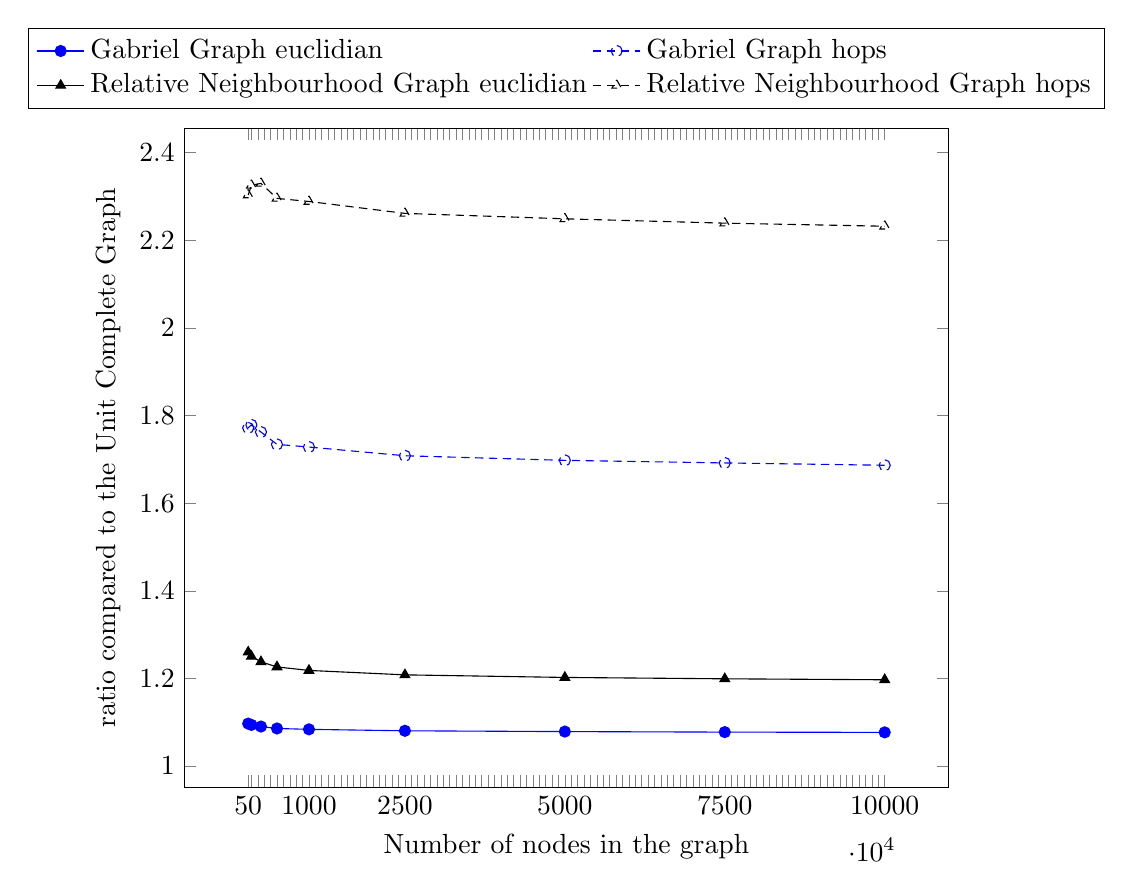
\begin{tikzpicture}
\pgfplotsset{every axis legend/.append style={at={(0.5,1.03)},anchor=south}}
\begin{axis}[scale only axis, xtick={50, 100, 200, 300, 400, 500, 600, 700, 800, 900, 1000, 1100, 1200, 1300, 1400, 1500, 1600, 1700, 1800, 1900, 2000, 2100, 2200, 2300, 2400, 2500, 2600, 2700, 2800, 2900, 3000, 3100, 3200, 3300, 3400, 3500, 3600, 3700, 3800, 3900, 4000, 4100, 4200, 4300, 4400, 4500, 4600, 4700, 4800, 4900, 5000, 5100, 5200, 5300, 5400, 5500, 5600, 5700, 5800, 5900, 6000, 6100, 6200, 6300, 6400, 6500, 6600, 6700, 6800, 6900, 7000, 7100, 7200, 7300, 7400, 7500, 7600, 7700, 7800, 7900, 8000, 8100, 8200, 8300, 8400, 8500, 8600, 8700, 8800, 8900, 9000, 9100, 9200, 9300, 9400, 9500, 9600, 9700, 9800, 9900, 10000}, xticklabels={$50$, , , , , , , , , , $1000$, , , , , , , , , , , , , , , $2500$, , , , , , , , , , , , , , , , , , , , , , , , , $5000$, , , , , , , , , , , , , , , , , , , , , , , , , $7500$, , , , , , , , , , , , , , , , , , , , , , , , , $10000$}, transpose legend, legend columns=2, width=0.8\linewidth, xlabel=Number of nodes in the graph, ylabel=ratio compared to the Unit Complete Graph, legend cell align=left]
\addplot[color=blue, mark=*] coordinates{                
(50, 1.0968)
(100, 1.0939)
(250, 1.0901)
(500, 1.0857)
(1000, 1.0837)
(2500, 1.0804)
(5000, 1.0786)
(7500, 1.0774)
(10000, 1.0768)
}; \addlegendentry{Gabriel Graph euclidian}
\addplot[color=black, mark=triangle*] coordinates{                
(50, 1.2600)
(100, 1.2503)
(250, 1.2378)
(500, 1.2262)
(1000, 1.2182)
(2500, 1.2081)
(5000, 1.2022)
(7500, 1.1991)
(10000, 1.1969)
}; \addlegendentry{Relative Neighbourhood Graph euclidian}
\addplot[color=blue, mark=o, densely dashed] coordinates{
(50, 1.7719)
(100, 1.7788)
(250, 1.7624)
(500, 1.7342)
(1000, 1.7282)
(2500, 1.7083)
(5000, 1.6978)
(7500, 1.6919)
(10000, 1.6866)
}; \addlegendentry{Gabriel Graph hops}
\addplot[color=black, mark=triangle, densely dashed] coordinates{
(50, 2.3036)
(100, 2.3257)
(250, 2.3301)
(500, 2.2958)
(1000, 2.2888)
(2500, 2.2616)
(5000, 2.2492)
(7500, 2.2393)
(10000, 2.2323)
}; \addlegendentry{Relative Neighbourhood Graph hops}
\end{axis}
\end{tikzpicture}
